\documentclass[a4paper]{article}



    \usepackage[colorinlistoftodos]{todonotes}
 
	\usepackage[utf8]{inputenc}
	\usepackage[T1]{fontenc}
    \usepackage[frenchb]{babel}
    \usepackage{textcomp} 
	\usepackage[top=3cm,left=3cm,right=3cm,bottom=2cm]{geometry}
    \usepackage{lmodern}
    \usepackage{sectsty}
    \usepackage{nicefrac}
	\usepackage{graphicx}
    \usepackage{lastpage}
    \usepackage{fancyhdr}
    \usepackage{amsmath}
    \usepackage{amssymb}
    \usepackage{amsfonts}
    \usepackage{capt-of}
    \usepackage{caption}
    \usepackage{tikz}
    \usepackage{multirow}
    \usepackage{todonotes}
    
    \usepackage{fancyvrb} % pour forcer les verbatim sur une seule page
    \usepackage{url}
    
    \usepackage{subfigure}
    \usepackage{minted}
    
    \newcommand\matlab{MATLab\textsuperscript{\textregistered}}

\renewcommand{\b}[1]{\boldsymbol{#1}}


\title{Compte rendu de TP: Formation de voies }

\author{Thomas Lechat \& Dinsenmeyer Alice}

\begin{document}
\maketitle



\section{Introduction}

La formation de voies est une méthode d'imagerie acoustique permettant d'obtenir la contribution de sources dans un plan à l'aide d'une antenne de microphones. 

Le principe général est de construire un vecteur de pointage qui pondère les signaux microphoniques en fonction du point d'observation sur le plan source.\\

Ce rapport vise à comparer trois méthodes de formation de voies testées sur des signaux microphoniques obtenus par des mesures de sources connues. 

\section{Obtention des données de test}

Des mesures de champs acoustiques sont effectuées à l'aide d'une antenne constituée de \textcolor{red}{??????} microphones disposés en spirale.

Les sources sont placées dans un plan situé à 1,43 m de l'axe de l'antenne. Deux configurations sont testées et présentées en figure~\ref{exp}.

\begin{figure}[!h]
	\subfigure[Configuration 1 : le haut-parleur 1 émet un sinus pur à 600 Hz et l'enceinte 2 émet un bruit blanc.]{
		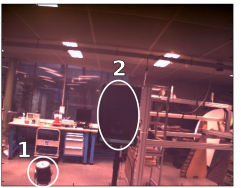
\includegraphics[width=.5\textwidth]{exp.png} }
	\hspace{1cm}
	\subfigure[Configuration 2 : le haut-parleur 1 émet un sinus pur à 800 Hz et l'enceinte 2 émet un bruit blanc.]{
		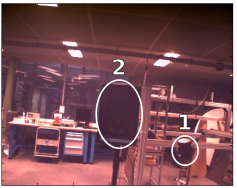
\includegraphics[width=.5\textwidth]{exp2.png}
	}
	\caption{\label{exp} Configurations du plan source.}
\end{figure}

La matrice interspectrale des microphones appelée $G_{pp}$ peut ainsi être obtenue à l'aide du logiciel Signal Express et du boîtier d'acquisition National Instrument.



\section{Méthode de Bartlet}

La méthode de Bartlet consiste à déterminer le vecteur de pointage $\b{w_i}$ tel que l'amplitude estimée des sources $S_i$ s'écrive : $$S_i=\b{w_{i}^{H}p},$$ avec $\b{p}$ les signaux de pression mesurés par les microphones.

Le vecteur $\b{w_i}$ est calculé en minimisant la fonction coût $|\b{w_{i}^{H}p}-A_i|$ où $A_{i}$ sont les amplitudes réelles des sources.

On trouve alors $$\b{w_{i}}=\b{\frac{h_i}{h_{i}^{H}h_{i}}}$$ avec $\b{h_i}$ la contribution de la source i, composée des fonctions de transfert entre chaque microphone m et cette source. Ces fonctions de transfert sont ici celles d'un rayonnement en espace libre sur une distance $r_{mi}$ : $$ h_{mi}=\frac{e^{-jkr_{mi}}}{4\pi r_{mi}}.$$


\section{Méthode de Capon}

Dans la méthode de Capon, seule la définition du vecteur de pointage change : on cherche à minimiser $\b{w_{i}^{H}G_{pp}w_{i}}$ avec la contrainte de normalisation $\b{w_{i}^{H}h_i}=1$. 

En résolvant ce problème avec la méthode des multiplicateurs de Lagrange, on trouve le nouveau vecteur de pointage suivant : $$\b{w_i=\frac{G_{pp}^{-1}h_{i}}{h_{i}^{H}G_{pp}^{-1}h_{i}}}.$$\\

Cette méthode est supposée donner de meilleurs résultats que la méthode précédente, mais comporte la contrainte de l'inversion de la matrice $G_{pp}$.

\section{Méthode MUSIC}

Cette méthode est basée sur la décomposition en valeurs propres de la matrice interspectrale $G_{pp}$. Cette matrice est ensuite décomposée en un sous-espace signal et un sous-espace bruit. Le sous-espace bruit correspond aux plus petites valeurs propres de $G_{pp}$ et est utilisé pour estimer la présence $P_i$ d'une source au point $i$ :
 \begin{equation}
 P_i = \frac{1}{\sum \limits_{q=r+1}^{M} \frac{\b{\left|h_{i}^{H}u_q\right|^{2}}}{\sigma_{p}^{2}}}
\end{equation}

où $\sigma_q$ sont les valeurs propres de l'espace bruit et $M$ est le nombre de champs cohérents orthogonaux qui composent $G_{pp}$.


\end{document}